\chapter{Introduction}

Drug (Figure \ref{Background:Drugs}) discovery is an industrial process, an expensive and long-term business, and a wasteful game. It takes about US\$1.8 billion over 13.5 years to develop a new drug \citep{716}. Out of 30,000 compounds synthesized, only 1 (0.003\%) makes a satisfactory ROI (Return On Investment) \citep{713}.

\begin{figure}
\centering
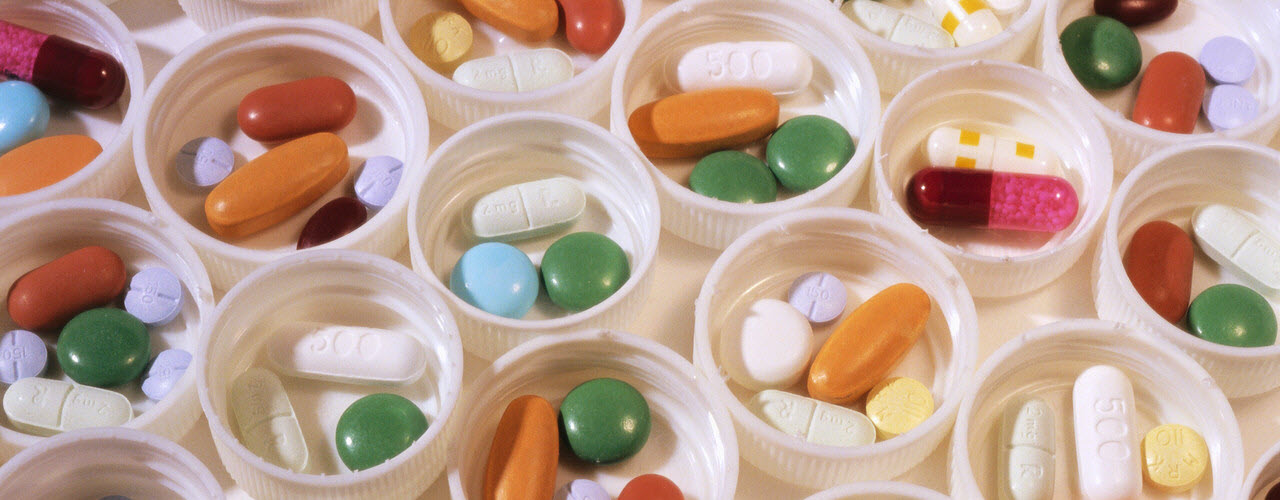
\includegraphics[width=\textwidth]{Background/Drugs.jpg}
\caption{Drugs.}
\label{Background:Drugs}
\end{figure}

\section{Motivation}

Drug discovery via biological and chemical means alone are both cost- and time-inefficient. Computer-aided drug discovery thus comes into the scene. Over recent decades, researchers have developed countless tools and utilities, and more are constantly emerging. We surveyed those tools and utilities, and summaried the major problems they suffer from. Generally speaking, they 1) are only commercially available, selling at a price that most small enterprises cannot afford, 2) are proprietary and closed source, making it difficult for others to learn inner implementation techniques and locate possible bugs, 3) conform to different standards and adopt different input/output formats because they are developed by separate teams, 4) require intensive and tedious configurations and lack fruitful documentations, an obstacle for others to set up the program properly, 5) run very slowly, using old-fashioned, blocking, single-threaded, low-performance programming style, or even worse, 6) are declared dead immediately upon their release due to zero maintenance afterward. Therefore, we are going to address these shortcomings.

\section{Objective}

Ultimately we aim to develop a comprehensive computational framework for structure-based drug discovery, simulating the early phases of modern drug discovery pipeline. Our framework shall 1) be free to the general public so that everyone can obtain it, 2) be released under permissive open source licenses so that everyone can study it, 3) be designed in conformance to a uniform and well-accepted standard so that everyone can use it with ease, 4) provide a SaaS (Software as a Service) platform with a HTML5- and CSS3-powered responsive web site so that everyone can play with it, 5) utilize multithreading and GPU acceleration to boost program execution so that everyone can really benefit from it, 6) track bugs, absorb user feedback, and release new versions regularly so that everyone can keep using it.

\section{Progress}

So far, we have developed idock for structure-based protein-ligand docking. We released idock 1.0 in July 2011. Compared with the state-of-the-art AutoDock Vina \citep{595}, idock 1.0 obtained a speed up of 6.3x to 10.4x, resulting in a screening performance of 1.3 drug-like ligands per CPU minute. We then released idock 1.1 in December 2011, idock 1.2 in February 2012, idock 1.3 in March 2012, and idock 1.4 in April 2012, further improving docking speed, adding new functionalities, and fixing bugs. idock 1.4 outperformed AutoDock Vina by 10x. With idock 1.4, we are now conducting massive protein-ligand docking experiements for our colleges and collaborators.

Moreover, on one hand, we are currently building a SaaS platform for idock in order to automate the protein-ligand docking process. On the other hand, we are working on computational ligand synthesis in order to discover novel potent compounds.

\section{Outline}

The thesis proposal is organized into 6 chapters as follows. Chapter 2 gives an overview of the pharmaceutial industry, and depicts the pipeline of modern drug discovery. Chapter 3 serves as a comprehensive literature survey on computer-aided drug discovery, and introduces several hot research problems we are currently working on. Chapter 4 presents our tool idock for structure-based protein-ligand docking. Chapter 5 describes our proposal, including two on-going projects, two in-plan projects, and several real case studies. Chapter 6 concludes the thesis proposal. Appendix A lists my publications.

\chapterend